\documentclass[]{article}

\usepackage{mathtools,mathrsfs,url,fancyhdr, graphicx,amssymb,esvect}

\renewcommand{\headrulewidth}{0pt}
\fancyhead[L]{}
\fancyhead[C]{
	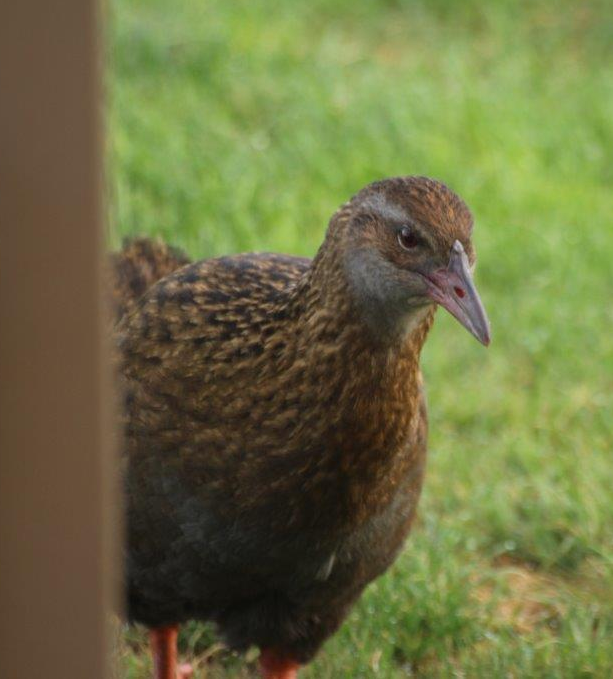
\includegraphics[width=2cm]{weka.png}
}



\graphicspath{ {images/} }
\newcommand{\Lagr}{\mathscr{L}}
\newcommand\numberthis{\addtocounter{equation}{1}\tag{\theequation}}
\pagestyle{plain}

%opening
\title{Introduction into General Relativity\\Assignment 3\\Problem 1\\The stress--energy tensor $T^{\mu\nu}$ for the dust}
\author{Simon Crase}

\begin{document}

\maketitle
\thispagestyle{fancy}


\section{Variation of the Action}

The Lecture Notes, \cite[(90)]{akhmedev2016}, give the following expression for the action of the dust.
\begin{align*}
S_M &= - \sum_{q=1}^N m_q \, \int d\tau_q \, \sqrt{g_{\mu\nu}[z_q(\tau_q)] \, \dot{z}_q^\mu(\tau_q)\, \dot{z}_q^\nu(\tau_q)}\\
&= - \int d^4 x \sum_{q=1}^N m_q \underbrace{\int d \tau_q \delta^{(4)} \big[x - z_q(\tau_q)\big]}_\text{As in \cite[(72)]{akhmedev2016}} \sqrt{g_{\mu\nu}[z_q(\tau_q)] \, \dot{z}_q^\mu(\tau_q)\, \dot{z}_q^\nu(\tau_q)} \\
&= - \int d^4 x \sum_{q=1}^N m_q \underbrace{\int d \tau \delta^{(4)} \big[x - z_q(\tau)\big] \sqrt{g_{\mu\nu}[z_q(\tau)] \, \dot{z}_q^\mu(\tau)\, \dot{z}_q^\nu(\tau)}}_\text{We can suppress the index on $\tau_q$ without confusion} \\
&\text{hence}\\
\delta_{g} S_M &= - \int d^4 x \sum_{q=1}^N m_q \int d \tau \delta^{(4)} \big[x - z_q(\tau)\big] \delta_{g} \big[\sqrt{g_{\mu\nu}[z_q(\tau)] \, \dot{z}_q^\mu(\tau)\, \dot{z}_q^\nu(\tau)}\big] \\
&= - \int d^4 x \sum_{q=1}^N m_q \int d \tau \delta^{(4)} \big[x - z_q(\tau)\big] \frac{ \dot{z}_q^\alpha(\tau) \dot{z}_q^\beta(\tau) \delta g_{\alpha\beta}}{2 \sqrt{g_{\mu\nu}[z_q(\tau)] \, \dot{z}_q^\mu(\tau)\, \dot{z}_q^\nu(\tau)}} \\
&= - \frac{1}{2} \int d^4 x \sum_{q=1}^N m_q \int d \tau \delta^{(4)} \big[x - z_q(\tau)\big] \frac{ \dot{z}_q^\alpha(\tau) \dot{z}_q^\beta(\tau) \delta g_{\alpha\beta}}{ \sqrt{g_{\mu\nu}[z_q(\tau)] \, \dot{z}_q^\mu(\tau)\, \dot{z}_q^\nu(\tau)}} \numberthis \label{eq:variation_of_action}
\end{align*}





\section{The Energy Momentum Tensor $T_{\mu\nu}$}



From the Lecture, \cite[(73)]{akhmedev2016}, $T_{\mu\nu}$ has the following definition:

\begin{align*}
\delta_g S_M =& \frac{1}{2} \int d^4 x \sqrt{|g|} T_{\mu\nu} \delta g^{\mu\nu} \numberthis \label {eq:T_def} \\
\text{Now}&\\
g_{\mu\rho}g^{\rho\sigma} =& \delta_{\mu}^{\sigma} \text{, where $\delta$ is the \emph{Kronecker} delta}\\
\delta g_{\mu\rho}g^{\rho\sigma} + g_{\mu\rho}\delta g^{\rho\sigma} =& 0 \text{, using $\delta$ to represent \emph{variation}}\\
\delta g_{\mu\rho}g^{\rho\sigma} =& - g_{\mu\rho}\delta g^{\rho\sigma}\\
\delta g_{\mu\rho}g^{\rho\sigma} g_{\sigma\nu} =& - g_{\mu\rho}\delta g^{\rho\sigma} g_{\sigma\nu} \\
\delta g_{\mu\nu} =& - g_{\mu\rho}\delta g^{\rho\sigma} g_{\sigma\nu} \numberthis \label {eq:useful_1}
\end{align*}

Combining (\ref{eq:T_def}) and (\ref{eq:useful_1}):
\begin{align*}
T^{\mu\nu}\delta g_{\mu\nu} =& - T^{\mu\nu} g_{\mu\rho}\delta g^{\rho\sigma} g_{\sigma\nu}\\
=& - T^{\mu\nu} g_{\mu\rho} g_{\sigma\nu} \delta g^{\rho\sigma}\\
=& -T_{\rho\sigma}\delta g^{\rho\sigma} \numberthis \label {eq:useful_2}
\end{align*}
Combining (\ref{eq:T_def}) and (\ref{eq:useful_2}):

\begin{align*}
\delta_g S_M =& - \frac{1}{2} \int d^4 x \sqrt{|g|} T^{\mu\nu} \delta g_{\mu\nu}\\
=& - \frac{1}{2} \int d^4 x \sum_{q=1}^N m_q \int d \tau \delta^{(4)} \big[x - z_q(\tau)\big] \frac{ \dot{z}_q^\alpha(\tau) \dot{z}_q^\beta(\tau) \delta g_{\alpha\beta}}{ \sqrt{g_{\mu\nu}[z_q(\tau)] \, \dot{z}_q^\mu(\tau)\, \dot{z}_q^\nu(\tau)}} \text{, from (\ref{eq:variation_of_action})}
\end{align*}
Comparing these two expressions for $\delta_g S_M$, they match \emph{iff}:

\begin{align*}
\sqrt{|g|} T^{\alpha\beta} =&  \sum_{q=1}^{N} m_q \int d\tau \delta^{(4)} \big[x-z_q(\tau)\big]\frac{\dot{z_q^\alpha} \dot{z_q^\beta}}{\sqrt{g_{\mu\nu}(z)\dot{z_q^\mu}\dot{z_q^\nu}}} \text{, whence} \\
T^{\alpha\beta} =& \frac{1}{\sqrt{|g|}} \sum_{q=1}^{N} m_q \int d\tau \delta^{(4)} \big[x-z_q(\tau)\big]\frac{\dot{z_q^\alpha} \dot{z_q^\beta}}{\sqrt{g_{\mu\nu}(z)\dot{z_q^\mu}\dot{z_q^\nu}}} \\
=& \frac{1}{\sqrt{|g|}} \sum_{q=1}^{N} m_q \int d\tau \delta^{(1)} \big[x^0-z^0_q(\tau)\big]\delta^{(3)} \big[\vv{x}-\vv{z_q}(\tau)\big]\frac{\dot{z_q^\alpha} \dot{z_q^\beta}}{\sqrt{g_{\mu\nu}(z)\dot{z_q^\mu}\dot{z_q^\nu}}} \numberthis \label{eq:T_penult}
\end{align*}

We know from \cite{wiki_delta} that:
\begin{align*}
\int_{-\infty}^{\infty} \delta(g(x)) f(x) dx  =& \sum_{x_i} \frac{f(x_i)}{|g'(x_i)|} \text{, summed $ \forall x_i$ such that $g(x_i)=0$}\\
&\text{so (\ref{eq:T_penult}) can be written}\\
 T^{\alpha\beta} =& \frac{1}{\sqrt{|g|}} \sum_{q=1}^{N} m_q  \delta^{(3)} \frac{\big[\vv{x}-\vv{z}_q(\tau)\big]}{|\dot{z}_q^0|}\frac{\dot{z_q^\alpha}  \dot{z_q^\beta}}{\sqrt{g_{\mu\nu}(z)\dot{z_q^\mu}\dot{z_q^\nu}}} \\
 T^{\alpha\beta} =& \frac{1}{\sqrt{|g|}} \sum_{q=1}^{N} m_q  \delta^{(3)} \frac{\big[\vv{x}-\vv{z}_q(\tau)\big]}{\dot{z}_q^0}\frac{\dot{z_q^\alpha}  \dot{z_q^\beta}}{\sqrt{g_{\mu\nu}(z)\dot{z_q^\mu}\dot{z_q^\nu}}}
\end{align*}
In the last step, we have used the fact that time $z^0$ increases with $\tau$ to replace $|\dot{z}_q^0|$ with $\dot{z}_q^0$.


Now $\sqrt{g_{\mu\nu}(z)\dot{z_q^\mu}\dot{z_q^\nu}}=s$, where s is the proper time.

\begin{align*}
T^{\alpha\beta}(x) =& \frac{1}{\sqrt{|g|}} \sum_{q=1}^{N} m_q \delta^{(3)} \frac{\big[\vv{x}-\vv{z}_q(s)\big]}{u_q^0 (s)} u_q^\alpha (s) u_q^\beta (s)  \numberthis \label{eq:T}\\
&\text{Where $u^{\mu} = \dot{z^\mu} = \frac{d z^\mu}{d s}$}
\end{align*}





\section{The Energy Density $\rho$}

\begin{align*}
\rho(x) =& T^{\mu\nu}(x) \, u_\mu(x) \, u_\nu(x) \text{, from \cite{wiki_dust}}\\
=& \frac{1}{\sqrt{|g|}} \sum_{q=1}^{N} m_q \delta^{(3)} \frac{\big[\vv{x}-\vv{z}_q(s)\big]}{u_q^0 (s)} u_q^\mu (s) u_q^\nu (s) u_\mu(x) u_\nu(x) \text{, from (\ref{eq:T})}\\
=&\frac{1}{\sqrt{|g|}} \sum_{q=1}^{N} m_q \frac{d z^0_q}{d s} \delta^{(3)} \big[\vv{x}-\vv{z}_q(s)\big] \numberthis \label{eq:density} \\
\frac{d z^0_q}{d s}=&\gamma \text{, relativistic correction}
\end{align*}


\begin{thebibliography}{9}
	
	\bibitem{akhmedev2016}
	Emil T. Akhmedev,
	\emph{Lectures on General Theory of Relativity},
	2016,
	\url{https://arxiv.org/pdf/1601.04996v6.pdf}.
	
	\bibitem{wiki_delta}
	Wikipedia,
	\emph{The Dirac Delta Function},
	\url{https://en.wikipedia.org/wiki/Dirac_delta_function#Composition_with_a_function},
	Retrieved: 4 April 2017
	
	\bibitem{wiki_dust}
	Wikipedia,
	\emph{Dust Solution},
	\url{https://en.wikipedia.org/wiki/Dust_solution#Mathematical_definition},
	Retrieved: 4 April 2017
\end{thebibliography}

\end{document}
